\section{Methodology}

%%%%%%%%%%%%%%%%%%%%%%%%%%%%%%%%%%%%%%%%%%%%%%%%%%%%%%%%%%%%%%%%%
\subsection{System Overview}

The system is first simplified into a beam with mass $m$, length $L$ and moment of inertia $I$. It has 2 independent spring and dampener systems, which represent the front and back wheels. It also have two person on the car frantically leaning acting as a pendulum with mass $m_p$, angle $\beta_A$ or $\beta_B$. A bumpy road is represented by a simple sine wave, and then the displacement of the front wheels can be represented by some function of time $f(t)$, and the displacement of the back wheels would be represented $f(t-\phi)$ where $\phi$ is the phase change in the sine function dependent on its wavelength and the length of the car. Compiling all this information, the system can be seen in Figure \ref{fig:system_overview}.

\begin{figure}[H]
    \centering
    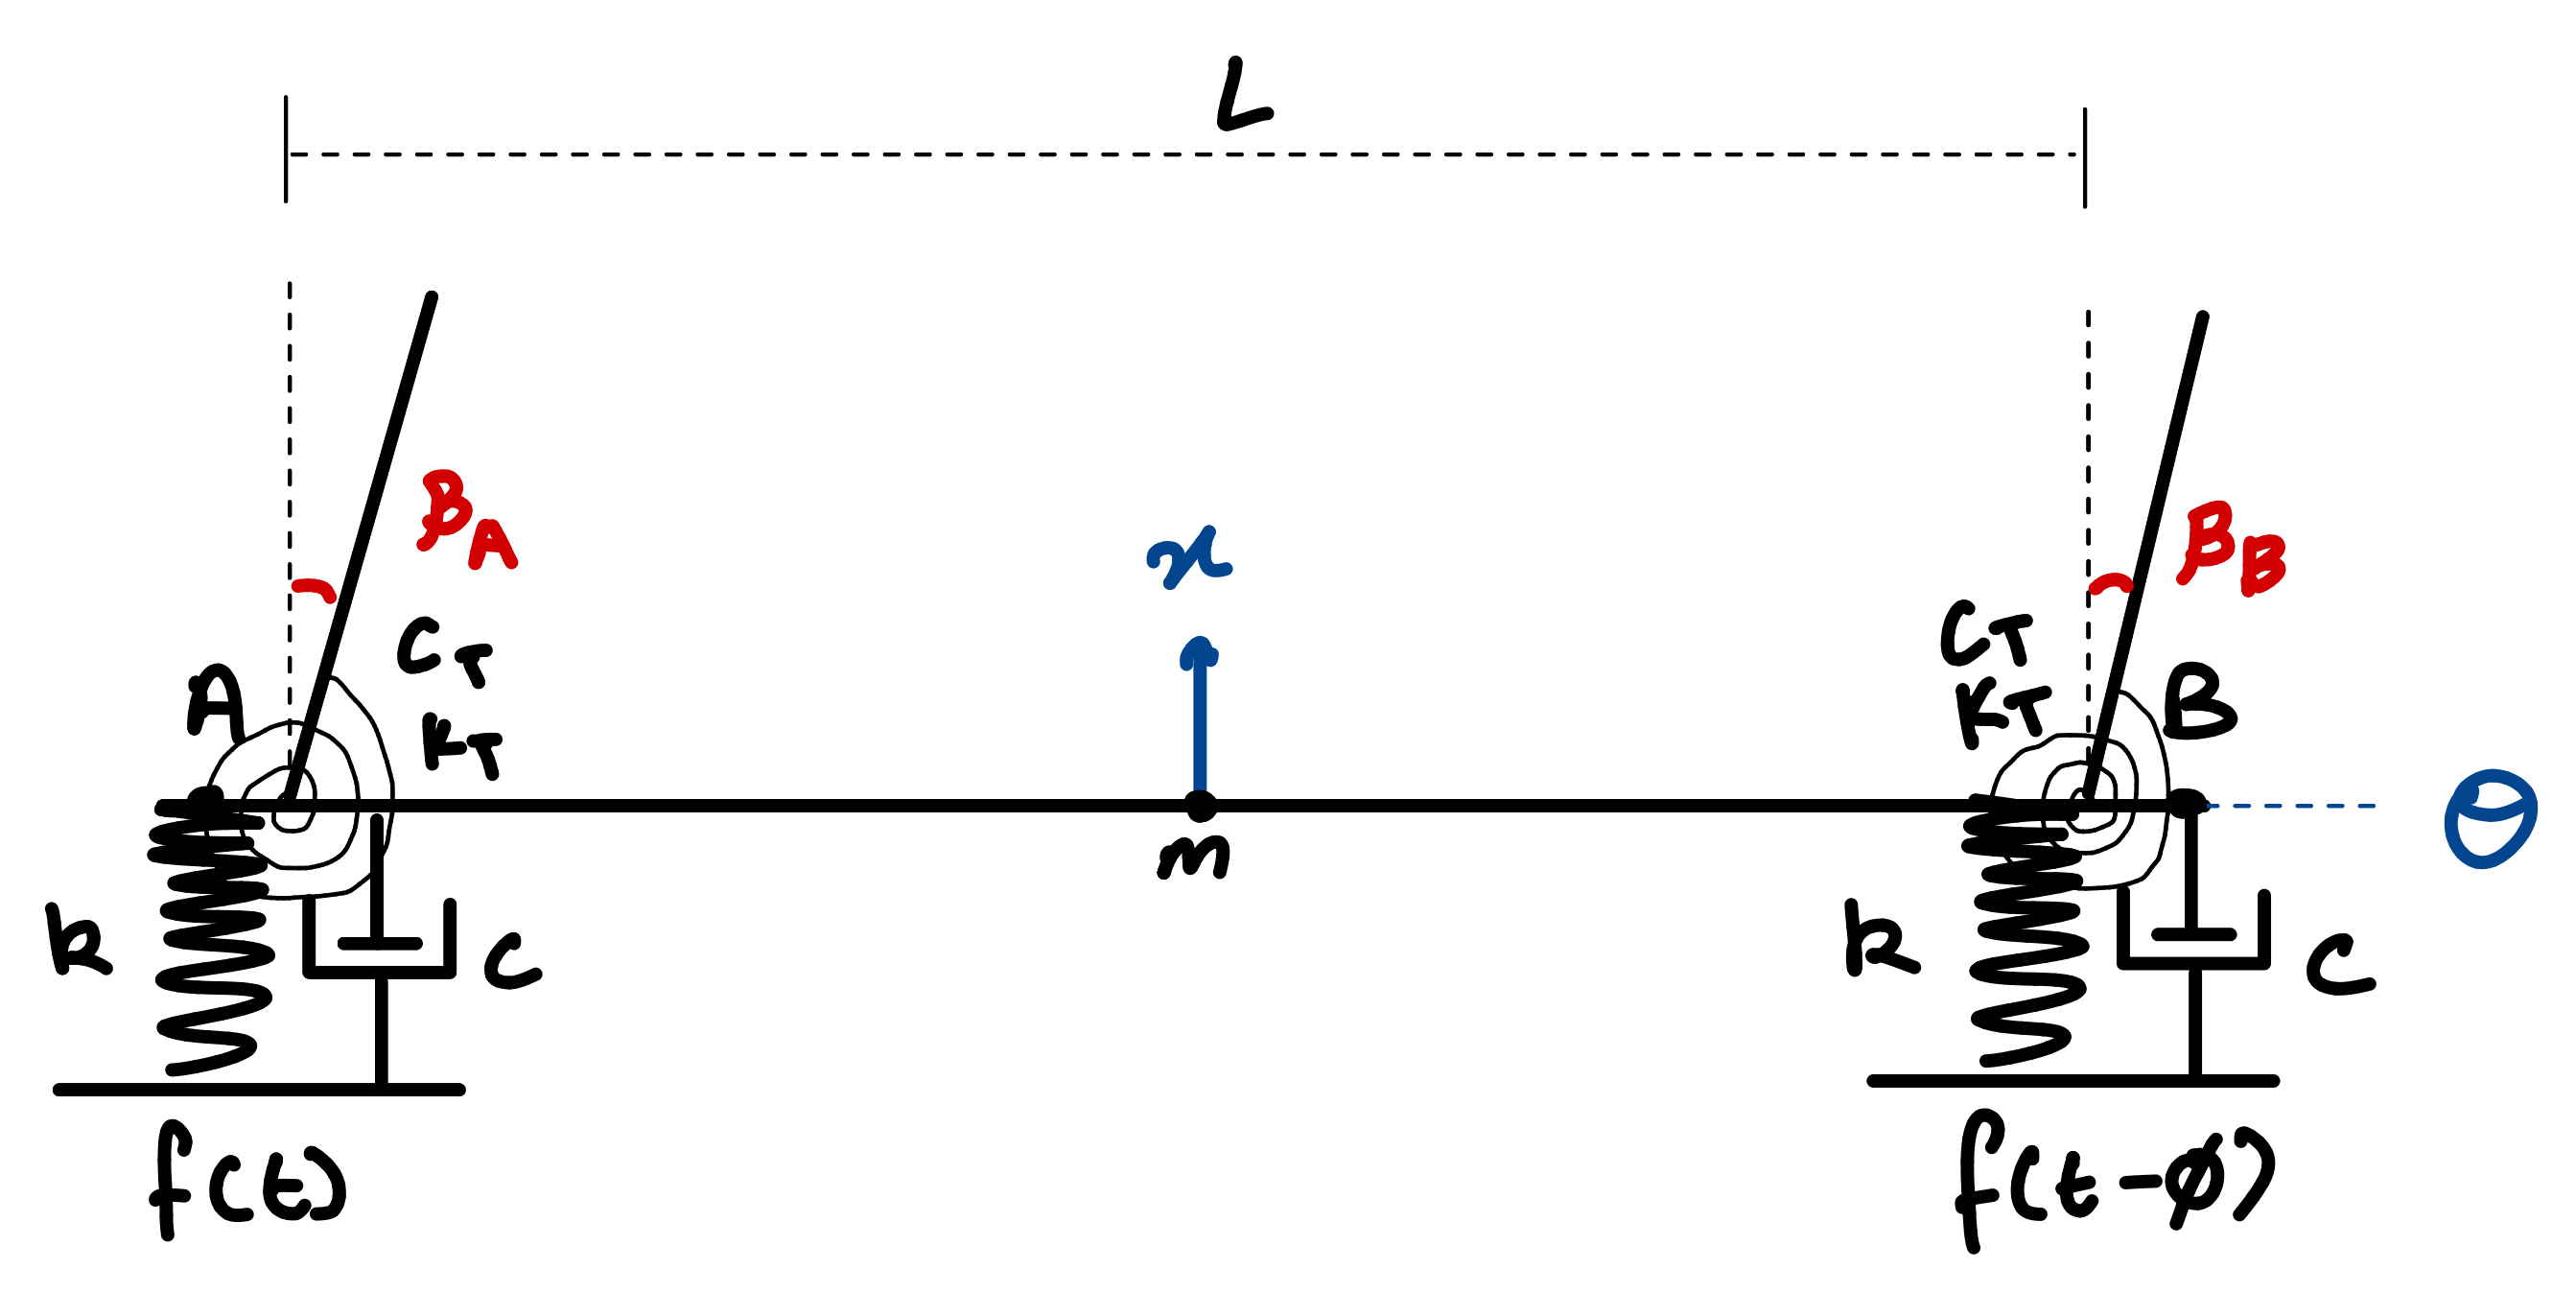
\includegraphics[width=0.6\linewidth]{Images/System_Overview.png}
    \caption{System Overview}
    \label{fig:system_overview}
\end{figure}

The goal of this task is to optimise the vertical displacement (x) and roll ($\theta$) of the car, which are the two degrees of freedom of the system. This is done by optimising the parameters of the spring and dampener systems, which are $K_{tor}$, $C_{tor}$,$k$ and $c$ respectively.

%%%%%%%%%%%%%%%%%%%%%%%%%%%%%%%%%%%%%%%%%%%%%%%%%%%%%%%%%%%%%%%%%
\subsection{Equations of Motion}

The system consists of one body in a 2-D plane. It has constraints in the horizontal axis, as that motion is defined by driving across the road, hence we are not going to consider that motion. Then the number of degrees of freedom (DoF) is as given below, where $N$ is the number of bodies and $k$ is the number of constraints.

\begin{equation*}
    DoF = 3N - k = 3-1 = 2
\end{equation*}

Hence, we require 2 equations of motion to fully define the motion of the system. These motions are $x$, which describes the vertical displacement, and $\theta$ which describes the roll of the body as shown in Figure \ref{fig:system_overview}.

We can then derive equations for $x$ and $\theta$ in terms of $a$ and $b$ which are the displacements for the attachment points for the 2 spring and dampener systems $A$ and $B$ respectively. From the geometry shown in Figure \ref{fig:system_geometry}, the equations of motion \ref{eq:theta_def} and \ref{eq:x_def} can be derived as shown.

\begin{figure}[H]
    \centering
    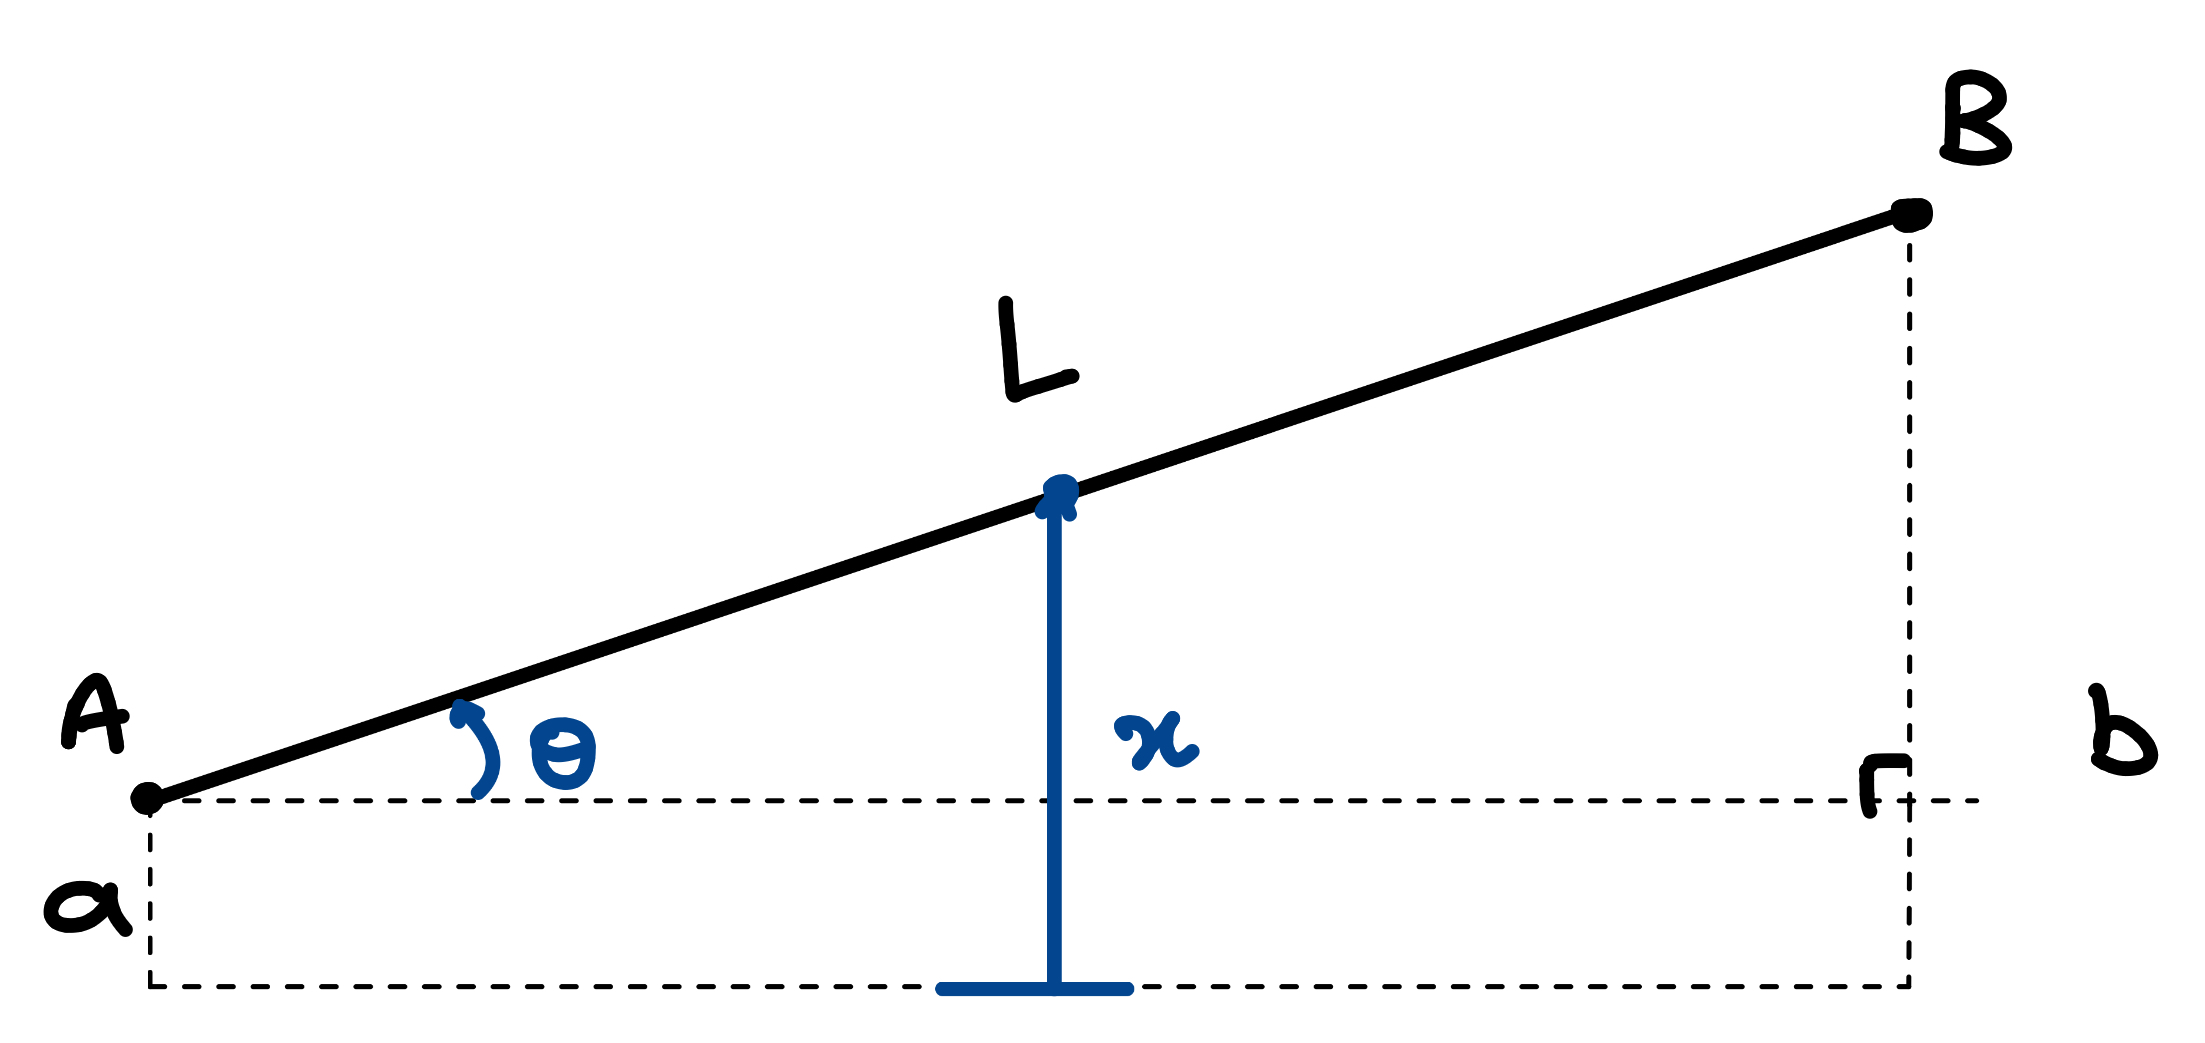
\includegraphics[width=0.6\linewidth]{Images/x_theta_geometry.jpeg}
    \caption{System Geometry}
    \label{fig:system_geometry}
\end{figure}

\begin{gather*}
    \sin(\theta) = \frac{b-a}{L} \\
    \implies \theta = \frac{b-a}{L} \quad \text{(small angle approximation)} \numberthis \label{eq:theta_def} \\
    x = a + \frac{L}{2}\theta = a + \frac{L(b-a)}{2L} \\
    \implies x = \frac{a+b}{2} \numberthis \label{eq:x_def}
\end{gather*}

Finally, using Newtonian Methods, we can find the net forces at $A$ and $B$ to get a coupled system of differential equations, and define the motion of the system. From the free body diagram (FBD) in Figure \ref{fig:fbd}, the equations in \ref{eq:a_eq_motion} and \ref{eq:b_eq_motion} can be derived as shown. Note, as the weight is a static force, the equilibrium position is taken where this force is balanced, and hence we only have to consider dynamic forces in the FBD.

\begin{figure}[H]
    \centering
    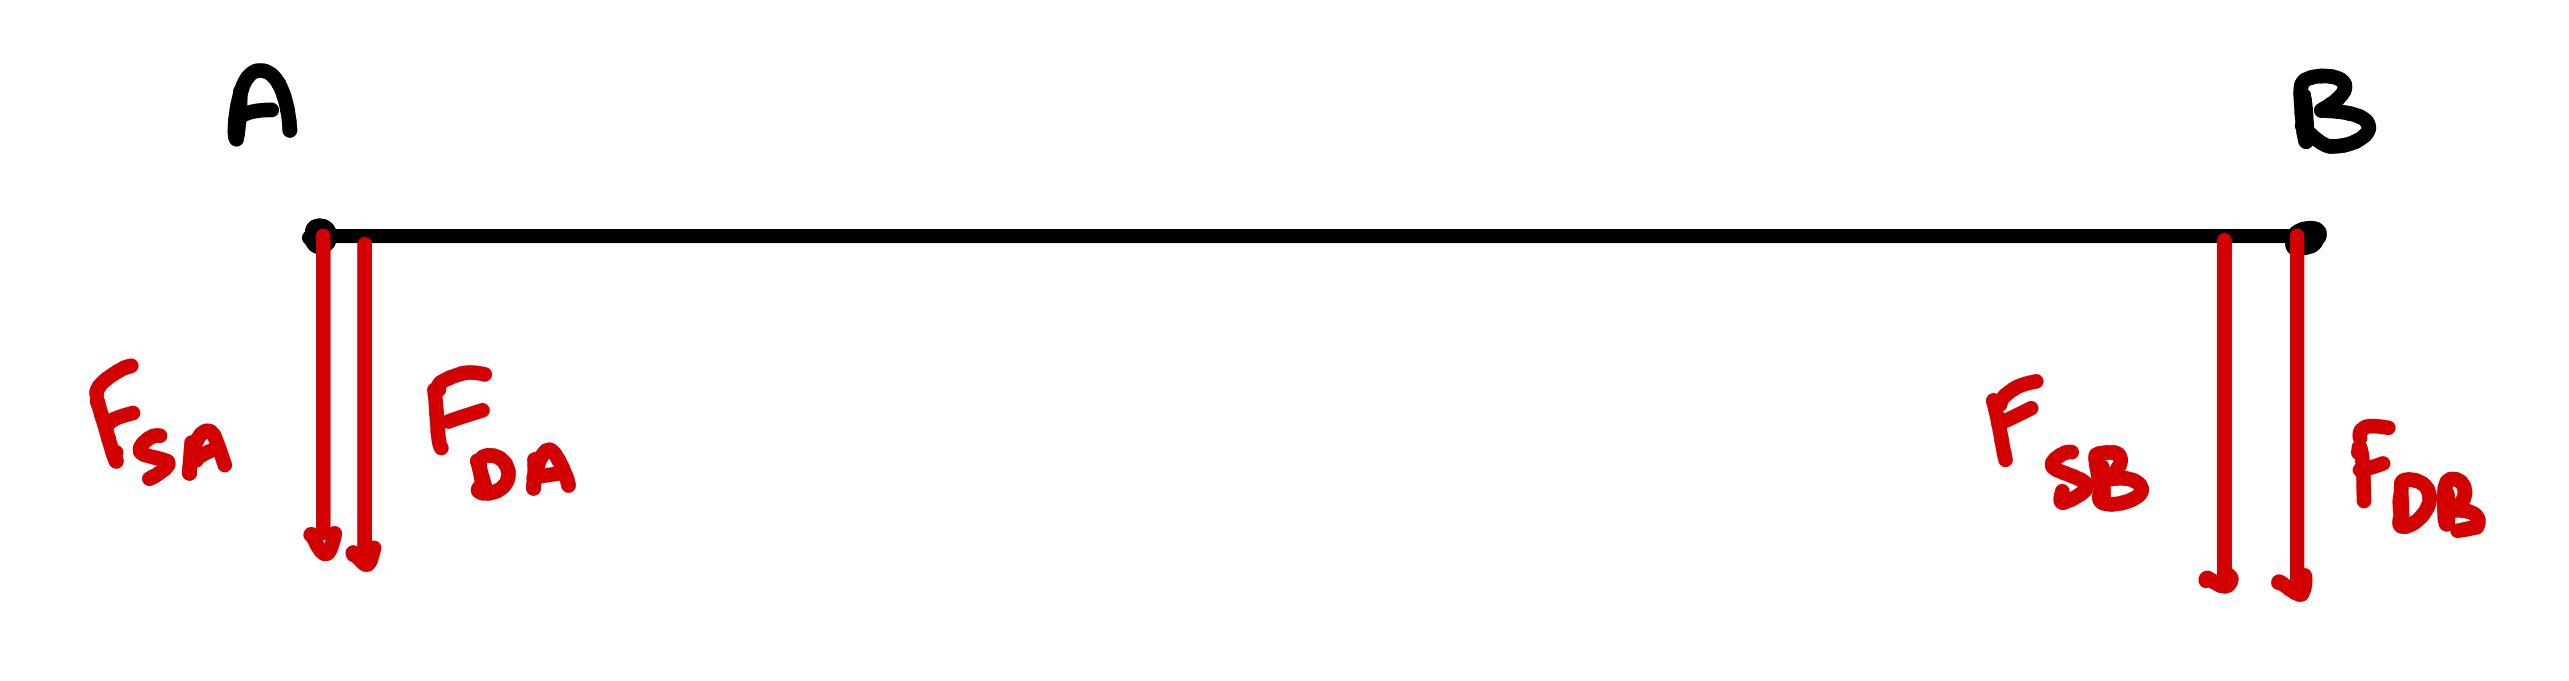
\includegraphics[width=0.6\linewidth]{Images/main_system_fbd.jpeg}
    \caption{Free Body Diagram of Dynamic Forces}
    \label{fig:fbd}
\end{figure}

\begin{gather*}
    \sum F_A = F_{sA} + F_{dA} \quad \text{and} \quad \sum F_B = F_{sB} + F_{dB} \\
    \implies m\ddot{a} = -k(a-f(t)) - c(\dot{a}-\dot{f}(t)) \quad \text{and} \quad m\ddot{b} = -k(b-\dot{f}(t-\phi)) - c\dot{b} \\
    \therefore m\ddot{a} + c\dot{a} + ka = kf(t) + c\dot{f}(t) \numberthis \label{eq:a_eq_motion} \\
    \text{and}~m\ddot{b} + c\dot{b} + kb = kf(t-\phi) + c\dot{f}(t-\phi)  \numberthis \label{eq:b_eq_motion} \\
    since \quad x = \frac{a+b}{2} \quad \text{and} \quad r(t) = f(t) \\
    m\ddot{x} + 2c\dot{x} + 2kx = k(r_A + r_B) + c(\dot{r}_A + \dot{r}_B) \numberthis \label{eq:x_eq_motion}
\end{gather*}

\subsubsection{Moments}

Taking moments about the centre of mass, the rotational equation of motion for $\theta$ is derived. The net moment contributions come from the spring-damper forces at attachment points $A$ and $B$, and the applied moments from the torsional pendulum restraints $M_{A_{p}}$ and $M_{B_{p}}$.

\begin{gather*}
    I\ddot{\theta} = \frac{L}{2}F_B - \frac{L}{2}F_A + M_{A_{p}} + M_{B_{p}} \\
    I\ddot{\theta} = \frac{L}{2}(F_B - F_A) + M_{A_{p}} + M_{B_{p}} \\
    I\ddot{\theta} = -2k\left(\frac{L}{2}\right)^2\theta - 2c\left(\frac{L}{2}\right)^2\dot{\theta} + \frac{L}{2}k(r_B - r_A) + ac(\dot{r}_B - \dot{r}_A) + M_{A_{p}} + M_{B_{p}} \\
    I\ddot{\theta} + 2c\left(\frac{L}{2}\right)^2\dot{\theta} + 2k\left(\frac{L}{2}\right)^2\theta = ak(r_B - r_A) + ac(\dot{r}_B - \dot{r}_A) + M_{A_{p}} + M_{B_{p}}
\end{gather*}

The applied moments from the torsional spring-damper at each pendulum attachment are:

\begin{gather*}
    M_{A_{p}} = k_{tor}\beta_A + C_{tor}\dot{\beta}_A \\
    M_{B_{p}} = k_{tor}\beta_B + C_{tor}\dot{\beta}_B
\end{gather*}

Substituting and combining gives the full rotational equation of motion:

\begin{gather*}
    I\ddot{\theta} + 2c\left(\frac{L}{2}\right)^2\dot{\theta} + 2k\left(\frac{L}{2}\right)^2\theta = ak(r_B - r_A) + ac(\dot{r}_B - \dot{r}_A) + k_{tor}(\beta_A + \beta_B) + C_{tor}(\dot{\beta}_A + \dot{\beta}_B) \numberthis \label{eq:theta_eq_motion}
\end{gather*}

\subsubsection{Pendulum}



%%%%%%%%%%%%%%%%%%%%%%%%%%%%%%%%%%%%%%%%%%%%%%%%%%%%%%%%%%%%%%%%%
\subsection{Computational Approach}

The system of differential equations was first put into sympy and simplified. Then they were solved numerically using the Runge-Kutta Method. A time step of $\Delta t = 0.01$ s was chosen to balance computational efficiency and accuracy.

The simulation was implemented in Python, and results were computed over a time span of 10 s.

%%%%%%%%%%%%%%%%%%%%%%%%%%%%%%%%%%%%%%%%%%%%%%%%%%%%%%%%%%%%%%%%%
\subsection{Constants and Initial Conditions}

The values for constants and initial conditions can be seen below. Other factors like $\phi$ are dependent on these and are calculated in the code.

\begin{gather*}
    v_0 = 5.6~\text{m/s} \\
    x_0 = 0~\text{m} \\
    \theta_0 = 0~\text{deg} \\
    L = 2.5~\text{m} \\
    m = 1200~\text{kg} \\
    f(t) = 0.025\sin(t) \\
\end{gather*}

%%%%%%%%%%%%%%%%%%%%%%%%%%%%%%%%%%%%%%%%%%%%%%%%%%%%%%%%%%%%%%%%%
\subsection{Validation and Convergence Testing}

To ensure the accuracy of the solution, convergence testing was performed by reducing the time step and plotting the residuals between results. Figure \ref{fig:convergence} shows how the results converge, indicating stability.

\begin{figure}[H]
    \centering
    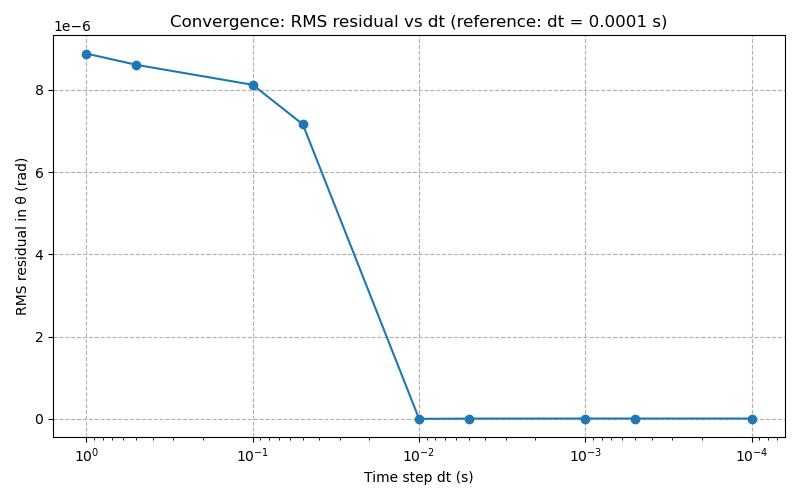
\includegraphics[width=0.6\linewidth]{Images/convergence_testing.png}
    \caption{Convergence Test}
    \label{fig:convergence}
\end{figure}

Then, the model was validated by simplifying the problem to drive on a flat road, and see how the system reacted. As shown in Figure \ref{fig:flat_tilt} and \ref{fig:flat_displacement}, the car is stable, which is what is expected on a flat road.

\begin{figure}[H]
    \centering
    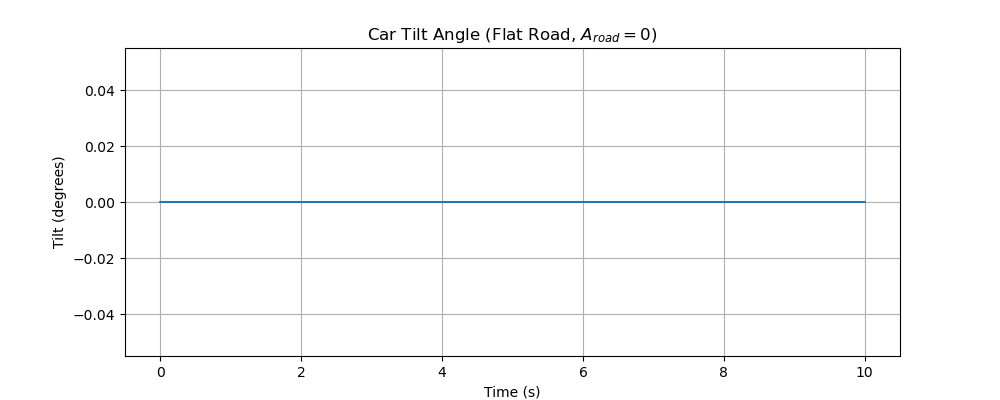
\includegraphics[width=0.6\linewidth]{Images/tilt_validation.png}
    \caption{Car Tilt on Flat Road}
    \label{fig:flat_tilt}
\end{figure}

\begin{figure}[H]
    \centering
    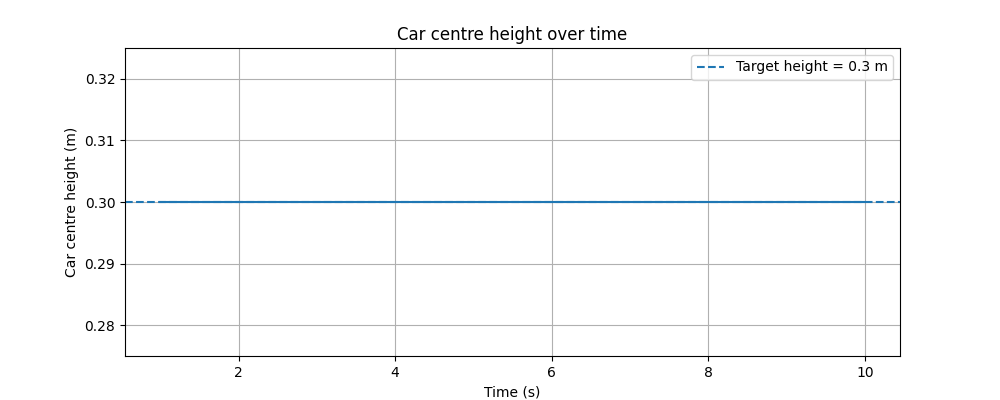
\includegraphics[width=0.6\linewidth]{Images/height_validation.png}
    \caption{Car Displacement on Flat Road}
    \label{fig:flat_displacement}
\end{figure}